\chapter{Problema del Interruptor Abierto}

\section{Interruptores analógicos}

Un interruptor analógico consiste en un transistor, normalmente de efecto de campo (FET), que se lleva a conducción o a saturación mediante una señal de control digital. Dado que el nivel y la velocidad de ésta pueden ser insuficientes para producir una transición rápida entre los dos estados, suele disponerse un activador entre la señal de control digital y el terminal de control del transistor.

\subsection{El interruptor ideal y el interruptor real}

En la figura \ref{fig:Interruptor Real} se presenta el modelo eléctrico de un interruptor analógico real, abierto y cerrado, en continua y en alterna, cuando consiste en un transistor FET; la adición de todos los elementos indicados permite considerar al interruptor $I$ como ideal. $I_S$ es la corriente de fugas del surtidor, $I_D$ es la de fugas del drenador y $R_{ON}$ es la resistencia entre drenador y surtidor en estado de conducción.

\begin{figure}[H]
    \centering
    \begin{subfigure}[c]{0.45\textwidth}
        \centering
        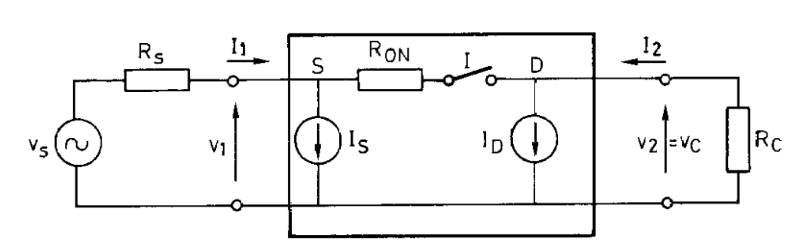
\includegraphics[width=\textwidth]{Imagenes/FET - Continua - Abierto.png}
        \caption{En continua, abierto}
    \end{subfigure}
    \begin{subfigure}[c]{0.45\textwidth}
        \centering
        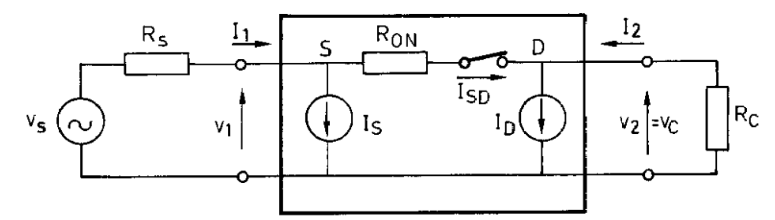
\includegraphics[width=\textwidth]{Imagenes/FET - Continua - Cerrado.png}
        \caption{En continua, cerrado}
    \end{subfigure}
    \begin{subfigure}[c]{0.45\textwidth}
        \centering
        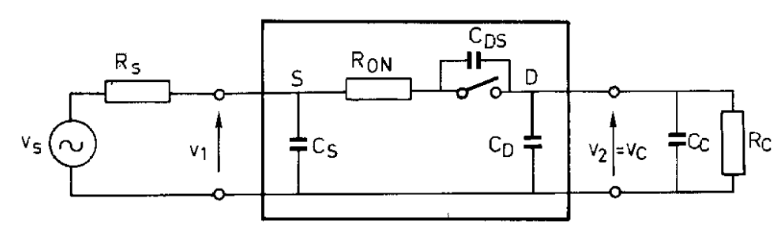
\includegraphics[width=\textwidth]{Imagenes/FET - Alterna - Abierto.png}
        \caption{En alterna, abierto}
    \end{subfigure}
    \begin{subfigure}[c]{0.45\textwidth}
        \centering
        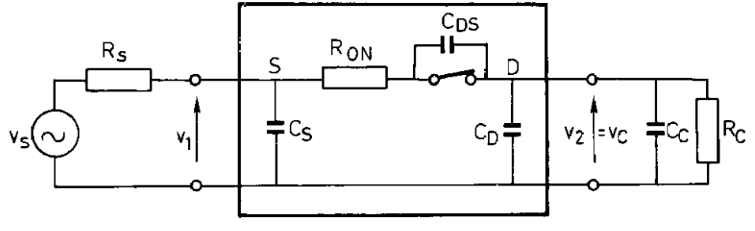
\includegraphics[width=\textwidth]{Imagenes/FET - Alterna - Cerrado.png}
        \caption{En alterna, cerrado}
    \end{subfigure}
    \caption{Modelos eléctricos para un interruptor real basado en un transistor FET.}
    \label{fig:Interruptor Real}
\end{figure}

\subsubsection{Errores en continua}
En corriente continua, cuando el interruptor está abierto la tensión de salida debería ser $v_2 = 0$, y sin embargo tenemos
\begin{equation}
    v_2 = -I_2 R_c = -I_D R_c
\end{equation}
Dado que la salida debería ser nula, no cabe hablar de error relativo. El error absoluto $E$ referido a la entrada $v_s$ es
\begin{equation}
    \frac{E}{v_s} = \frac{v_2 - 0}{v_s}
\end{equation}
Cuando el interruptor está cerrado deberíamos tener $v_2 = v_1 = v_s$, e $I_1 = 0$, y sin embargo tenemos
\begin{equation}
    I_1 = I_S + I_SD = I_S + I_D - I_2
\end{equation}
\begin{equation}
    v_2 = -I_2 R_c \approx \frac{v_s}{R_S + R_{ON} + R_C} R_C 
\end{equation}
Hay, pues, un error relativo
\begin{equation}
    \varepsilon \approx \frac{v_s - v_s}{v_s} = \frac{- (R_S + R_{ON})}{R_S + R_{ON} + R_C}
\end{equation}

Dado que tanto $I_S$ como $I_D$ son muy pequeñas, y a la vez $R_C$ puede ser fácilmente $1M\Omega$ los errores que se cometen en continua cuando se emplean interruptores FET son muy pequeños. Al factor $R_C/(R_C + R_{ON})$ se le denomina pérdidas por inserción, IL, (Insertion Loss), y se expresa en decibelios

\begin{equation}
    IL (dB) = 20 log \frac{R_C}{R_C + R_{ON}}
\end{equation}

\subsubsection{Errores en alterna}

Cuando la señal de entrada al interruptor es alterna, hay que tener en cuenta las capacidades parásitas del interruptor y de la carga. La presencia de capacidades parásitas afecta por una parte al tiempo de respuesta (tiempo de establecimiento, settling time) en la apertura y cierre, y al aislamiento entrada-salida cuando el interruptor está abierto.

El error relativo que se comete al medir la salida en un instante $t$ será

\begin{equation}
    \varepsilon = \frac{v_o(t) - v_i(t)}{v_i(t)} = \frac{-\frac{1}{1+\omega^2 \tau^2} exp(-t/\tau) + \frac{1}{(1 + \omega^2 \tau^2)^{1/2}} cos(\omega t - \theta)}{cos(\omega t)} - 1
\end{equation}

y, por lo tanto, depende no sólo del factor $t/\tau$ como sucede para una entrada continua, sino también de $\omega\tau$.

\subsubsection{Velocidad de conmutación}

En un interruptor ideal la apertura y el cierre del circuito son inmediatos. En un interruptor real hay un retardo desde que se da la orden, en forma de señal digital, hasta que se alcanza la situación final en el canal. Este retardo suele especificarse mediante el denominado tiempo de conmutación, $t_c$, que se define para una señal de entrada $v_s$ constante (positiva o negativa).

%\section{Parámetros característicos de los contactos}

%\section{Multiplexores Analógicos y Digitales}

%\subsection{Errores de offset por corrientes de fuga}

%\subsection{Errores en alterna}

%\subsection{Errores en conmutación}

%\subsection{Errores de control}

\subsection{Parámetros de los interruptores analógicos}

Los parámetros de los interruptores analógicos se pueden agrupar según se regieran al contacto (impedancai, entrada, salida), a la conmutación, al control de la conmutación, y a las características ambientales, incluida la alimentación.

\begin{itemize}
    \item Características del contacto.
    \begin{itemize}
        \item $R_{ON}$ : $R_{DS}$, resistencia óhmica entre surtidor y drenador cuando está cerrado; varía con la señal, la alimentación y la temperatura. El valor y la dependencia con la señal decrecen para tensiones de alimentación altas y temperaturas bajas.
        \item $\Delta R_{ON}$: diferencia entre $R_{ON}$ para interruptores con un mismo encapsulado.
        \item $I_{DS}$: corriente (máxima) a través del interruptor cerrado. Se especifica un valor para corriente continua y otro para alterna.
        \item $I_D$, $I_S$: corrientes respectivas en los terminales D o S.
        \item $C_D$, $C_S$: capacidad respectiva entre los terminales D o S, y la masa (terminal de referencia). Dependen de la condición ON/OFF.
        \item $C_{DS}$: capacidad entre los terminales D y S. Determina el aislamiento.
        \item $C_{DD}$, $C_{SS}$: capacidad entre los terminales D y entre los terminales S de distintos interruptores en un mismo encapsulado. Influye en la diafonía entre canales.
    \end{itemize}
    \item Características de conmutación.
    \begin{itemize}
        \item $t_{ON}$: retardo entre el 50\% de la señal de control y el instante cuando se considera que el interruptor está cerrado.
        \item $t_{OFF}$: retardo entre el 50\% de la señal de control y el instante cuando se considera que el interruptor está abierto. 
        \item Operación bbm o mbb: En interruptores dobles, la apertura del circuito precede al cierre del otro (operación bbm -\textit{break before make}-) o al revés (operación mbb -\textit{make before break}-).
    \end{itemize}
    \item Características de control.
    \begin{itemize}
        \item $V_{INL}$: tensión umbral para tener el estado <<bajo>>.
        \item $V_{INH}$: tensión umbral para tener el estado <<alto>>.
        \item $I_{INL}, I_{INH}$: corriente respectiva en la entrada de control.
        \item $C_{IN}$: capacidad entre la entrada digital y masa.
        \item Inyección de carga: carga inyectada desde el terminal de control a la salida.
    \end{itemize}
\end{itemize}